\chapter{Directional Noise Elimination}\label{ch:directional}
\section{Introduction}
This chapter deals with directional filtering. The idea is presented and tested. The 
results and conclusions will be shown afterwards.
\section{Concept}
Figure \ref{fig:2sources} shows a scenario where directional filtering could be used.
Source 1 and Source 2 are both talking simultaneously. At the Origin, two microphones 
left (L) and right (R) are recording both signals.

\begin{figure}[htp]
	\centering
	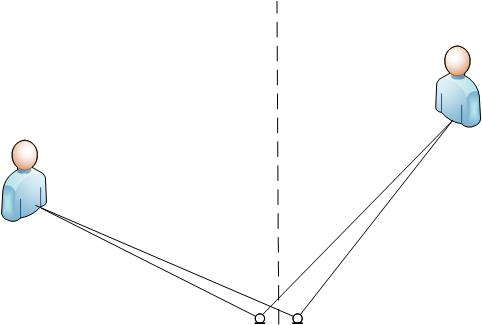
\includegraphics[width=0.65\textwidth]{Illustrations/2sources.jpg}
	\caption{Two Persons Talking}
	\label{fig:2sources}
\end{figure}

Due to the placement of the sources, both microphones will record the sounds, with a 
certain delay.

\section{Idea for filtering}

\begin{figure}[htp]
	\centering
	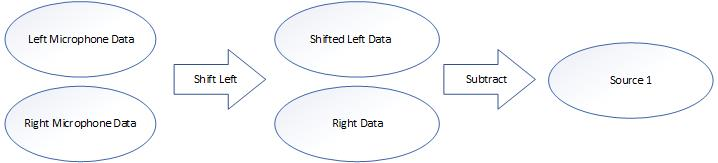
\includegraphics[width=1\textwidth]{Illustrations/IdeaDiagram.jpg}
	\caption{Idea diagram}
	\label{fig:IdeaDiagram}
\end{figure}

Filtering sound, based on the direction that it's coming from could work by taking data, recorded by one of the microphones, in this case (figure
\ref{fig:IdeaDiagram}) we chose left microphone data. Then we shift this data by exact amount of samples, which would make the source we would like 
to separate recorded by left microphone, exactly aligned with same source, recorded by right microphone.\\
Then by subtracting right microphone data from shifted left, we should get all the other sounds except the ones from source we would like to
separate, this is what we will call noise in directional filtering.\\
Separating could be done by taking the original data, putting it to one channel. Then subtracting noise from the original data should leave us only
with "clean" sound from the direction, we are interested in.\\
\section{Development}
\todo{MENTION WHERE EACH SUBSECTION COMES IN PLAY}
\subsection{Finding delay in samples}
By setting the angle of what we want to separate our signal at, we can calculate how big shift in samples that would account for. We are using this 
delay later, in the directional filtering. Calculations involve using selected angle, gap between microphones, sampling frequency of used 
microphones and the 
speed of sound. \\
\todo{DO WE WRITE ABOUT MATH AND EQUATIONS IN MATLAB HERE OR DO WE JUST SKIP IT.}
\subsection{Recording samples}
First, in order to record two microphones in separate tracks directly to computer, we need to give access to multiple inputs and outputs,  
independently to computers' sound card. To achieve that audio driver caller ASIO4ALL was used. Using this driver, together with recording software, 
which supports multiple input recording, we were able to record different situations with two microphones at the same time. \\
\todo{process of setting up for first recordings. Last sentence counters delay paragraph in Filtering section (4.3.3)}
Recording with two microphones was set in a quiet room with sound panels on the walls and curtains, all of 
which reduces echo. Using ruler as a guide microphones were set in place and then angles were marked as 
guides to know from which direction sound is coming from. (Figure \ref{fig:recSetup}) 
\begin{figure}[htp]
	\centering
	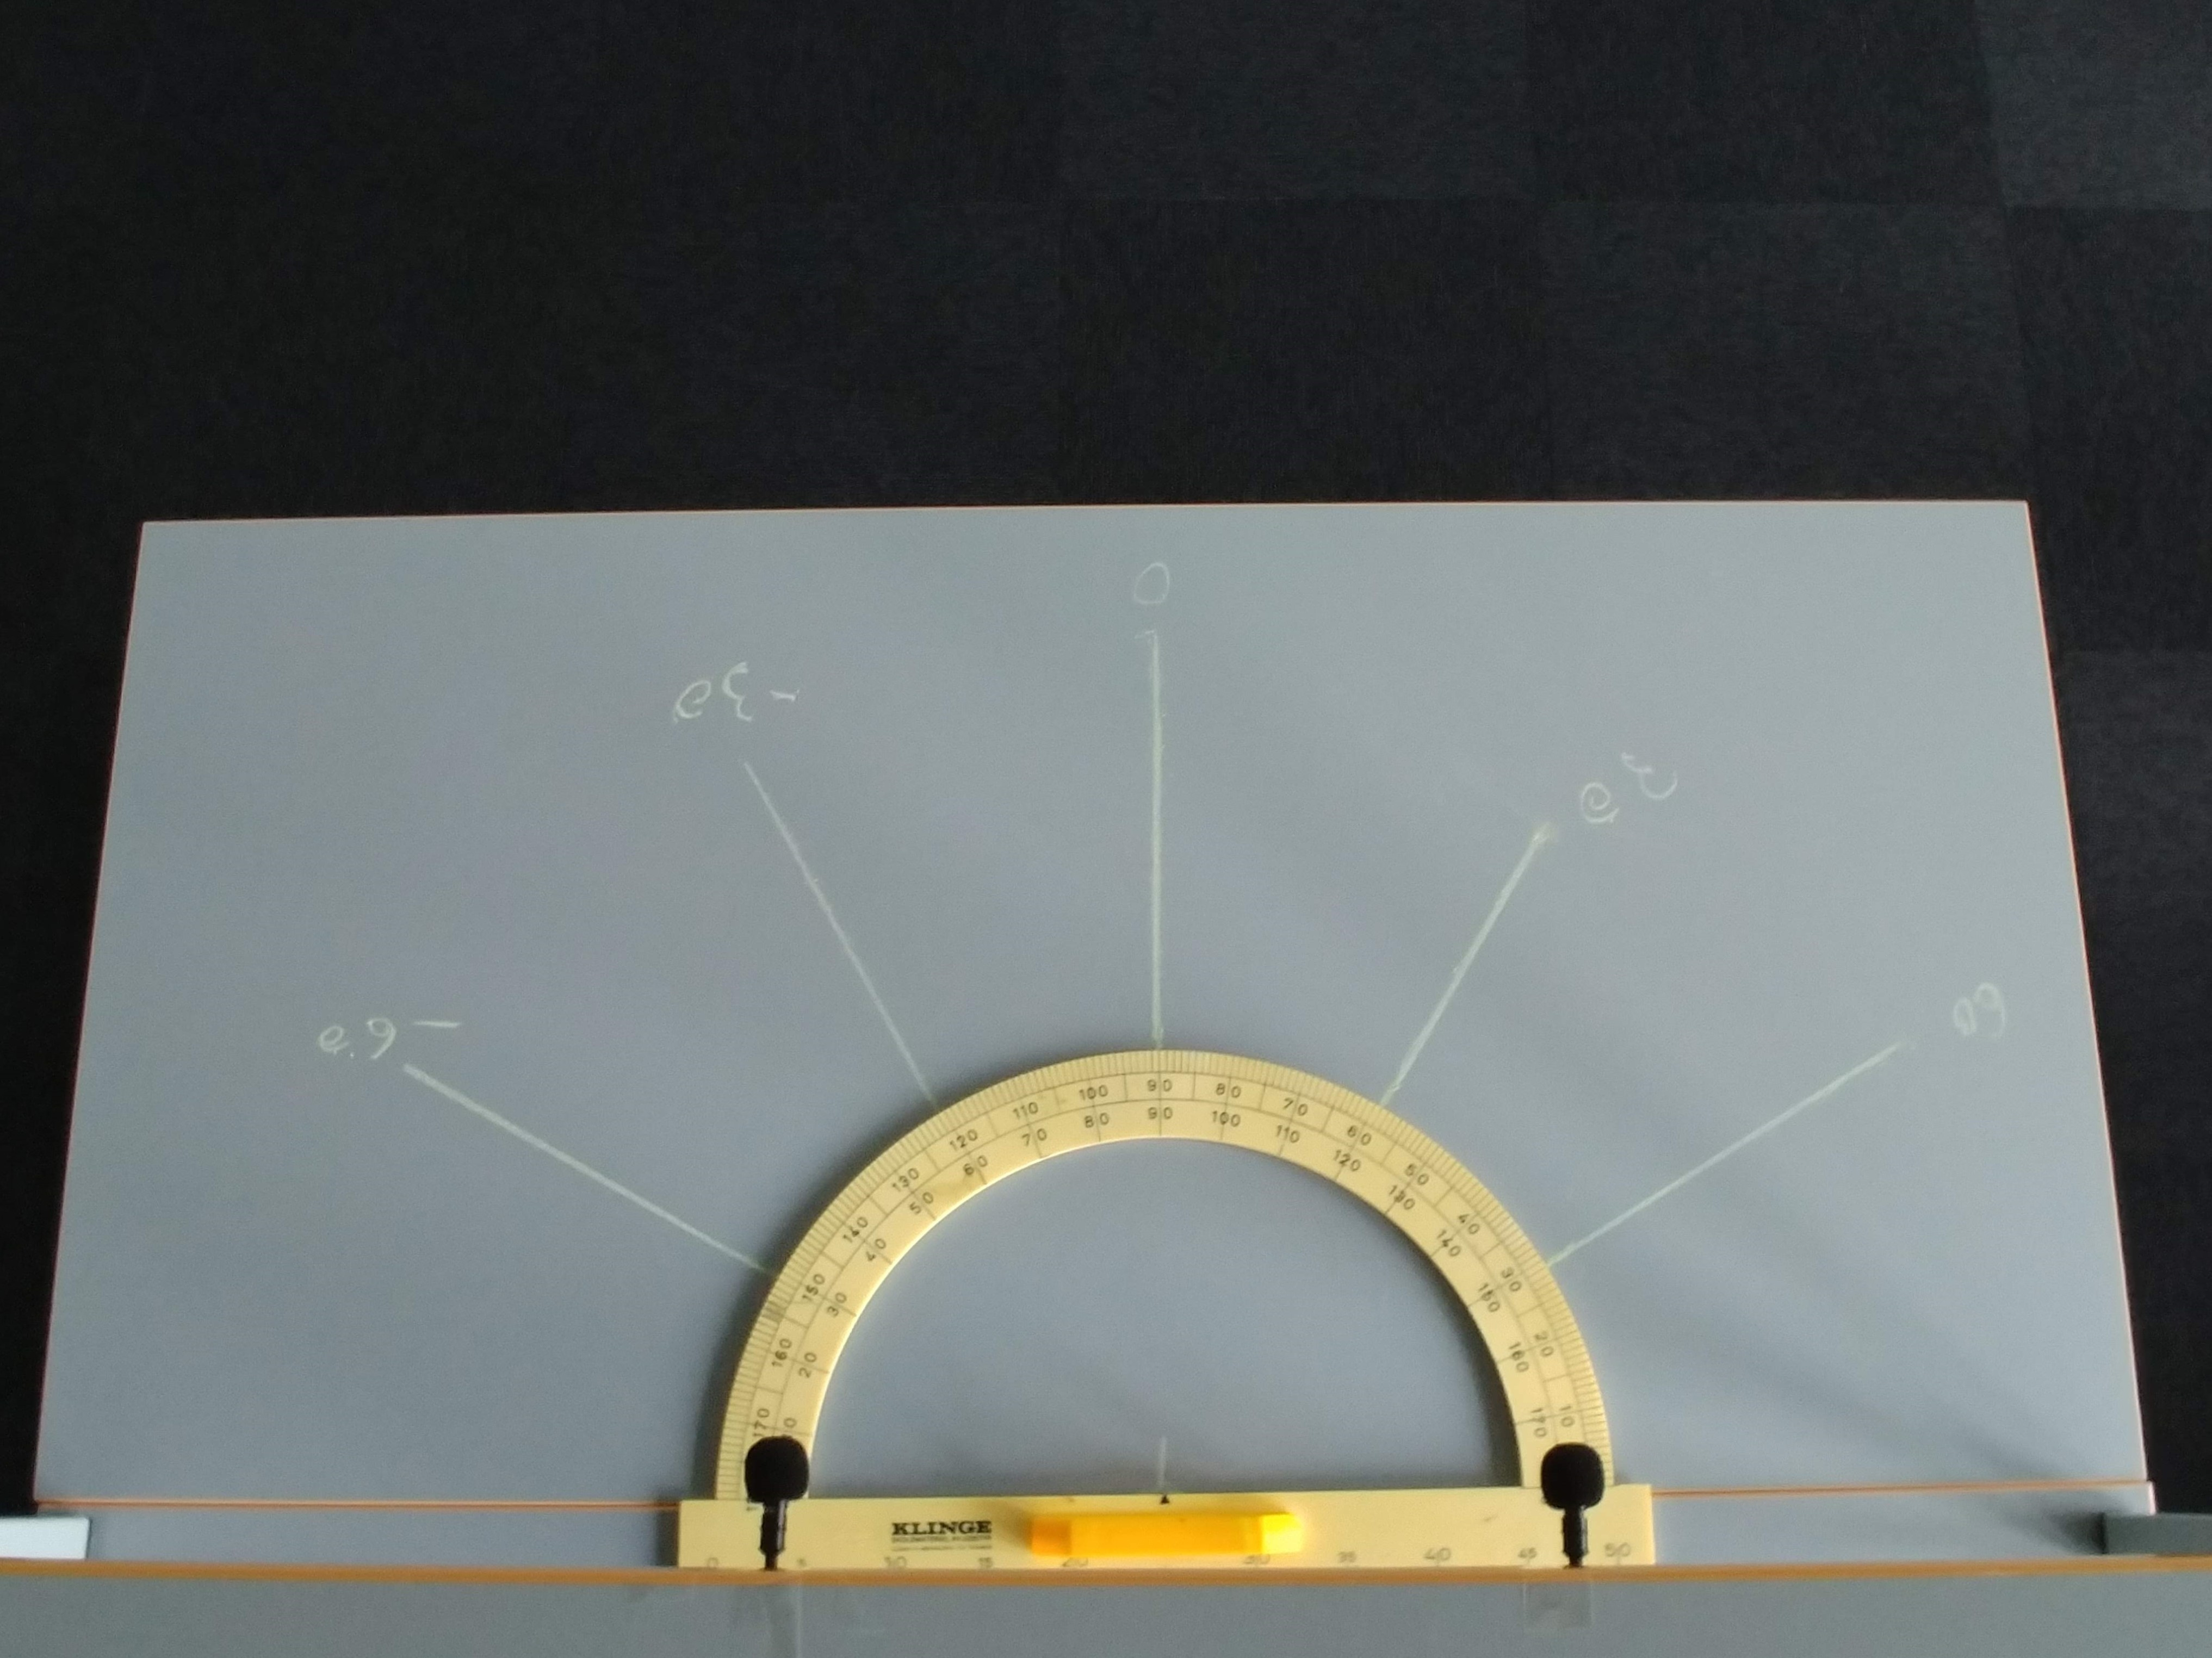
\includegraphics[width=1\textwidth]{Illustrations/JustSetup.jpg}
	\caption{Setup for recording}
	\label{fig:recSetup}
\end{figure}




\subsection{Filtering}
All of the directional filtering is done by applying the logic discussed before to the Matlab script.\\
Prior to shifting signals and filtering, we had to remove any delays, induced by hardware or software. This 
issue was resolved by starting every recording with loud, sharp sound like a clap or a finger snap right in 
the middle of the microphones. Using this sound in the beginning we could match loudest peaks, thus 
eliminating hardware and software induced delay. \\
To see if we can get the samples, which show that logic behind direction of delay is correct, we set up a 
recording with just one person first see figure \ref{fig:RanzvanRecSetup}.\\

\begin{figure}[htp]
	\centering
	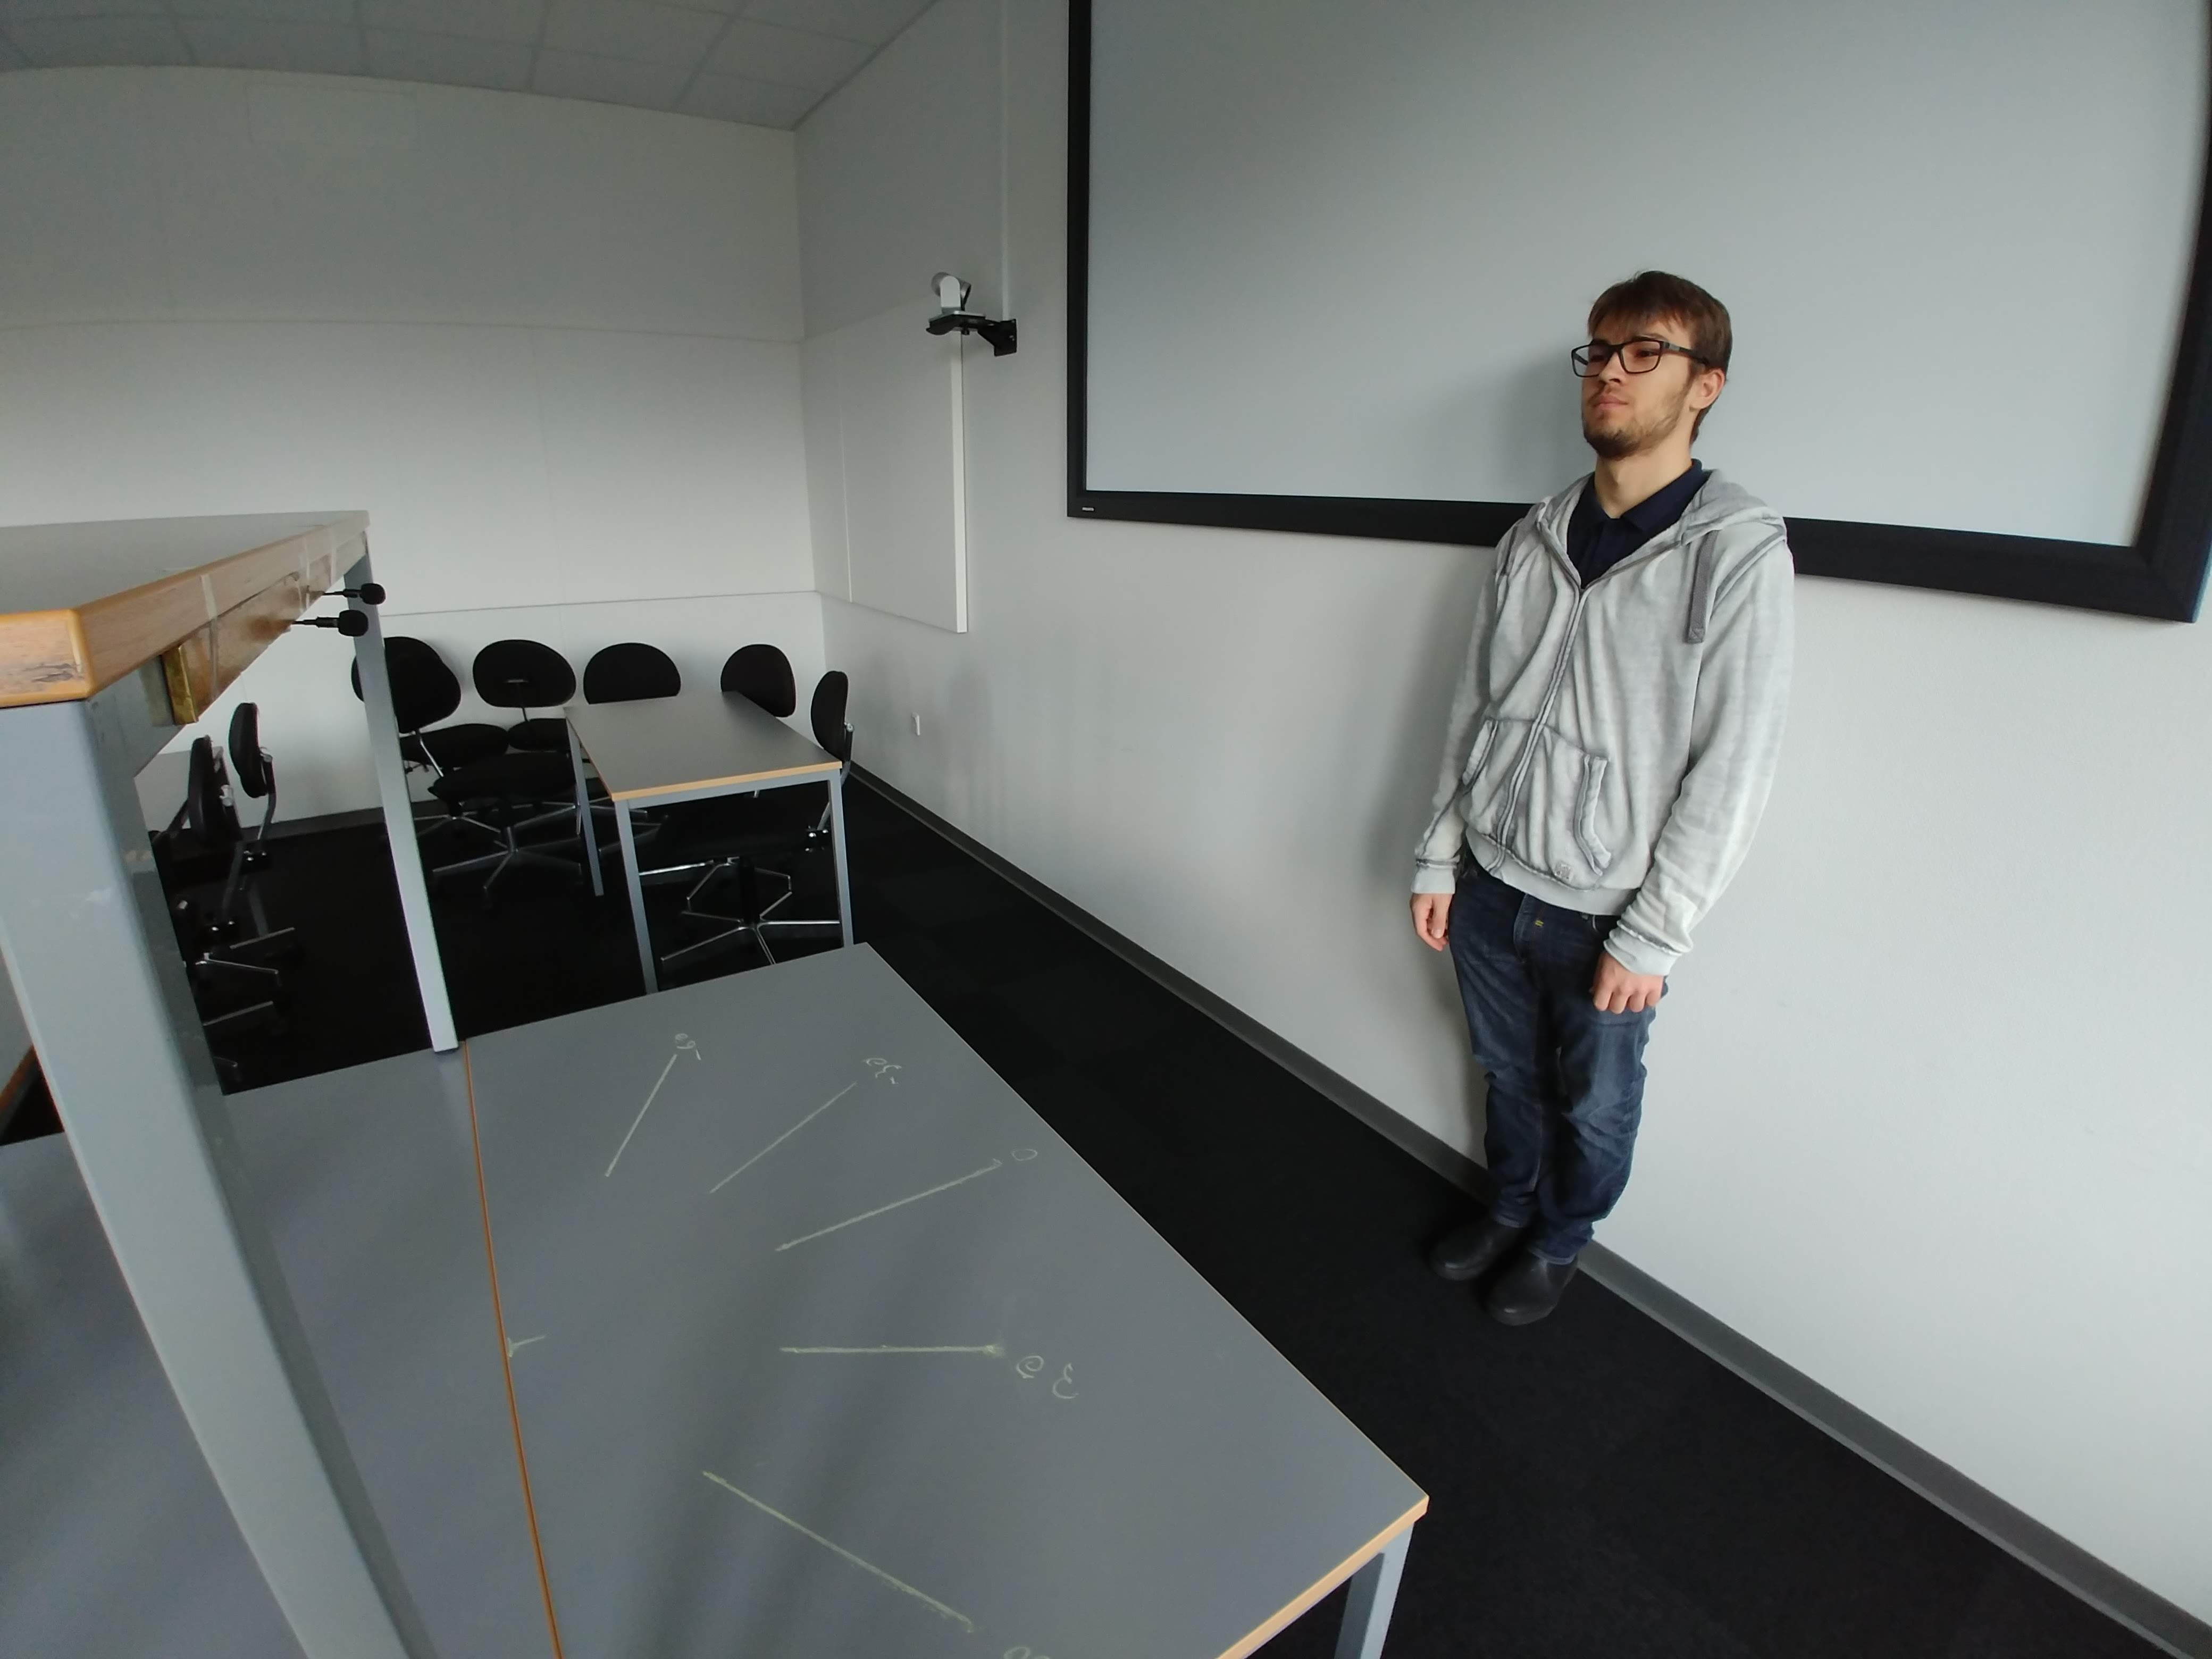
\includegraphics[width=0.8\textwidth]{Illustrations/razvanWithSetup.jpg}
	\caption{Setup for recording with a person}
	\label{fig:RanzvanRecSetup}
\end{figure}

Then we looked at data, collected:\\
When person spoke from the center, recordings (Figures  \ref{fig:C}, \ref{fig:closeC}) show that recordings 
match in phase.\\

\begin{figure}[htp]
	\centering
	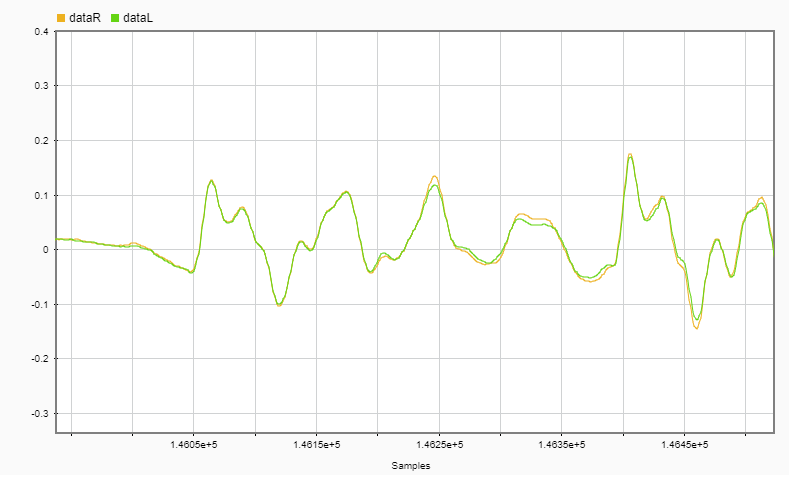
\includegraphics[width=0.8\textwidth]{Illustrations/DataC.png}
	\caption{Data from speaker in the center}
	\label{fig:C}
\end{figure}

\begin{figure}[htp]
	\centering
	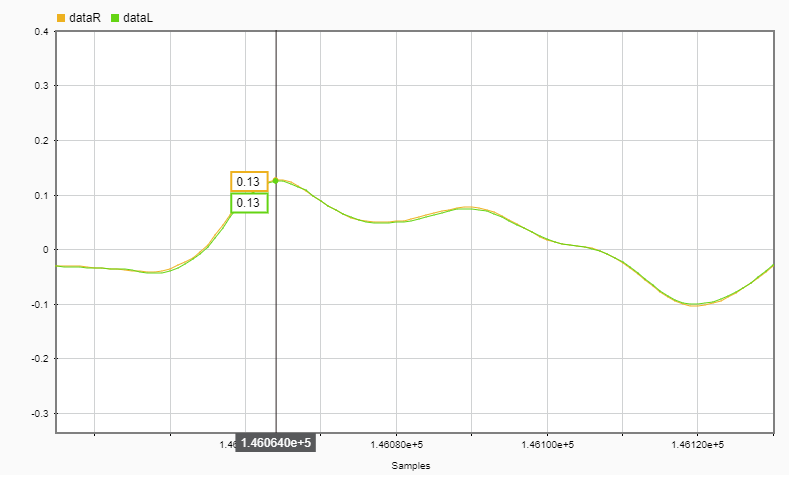
\includegraphics[width=0.8\textwidth]{Illustrations/DataC_with_Markers.png}
	\caption{Zoomed in data from speaker in the center}
	\label{fig:closeC}
\end{figure}
When person spoke from the right, right microphone data led left microphone (Figures  
\ref{fig:R}, \ref{fig:closeR})\\

\begin{figure}[htp]
	\centering
	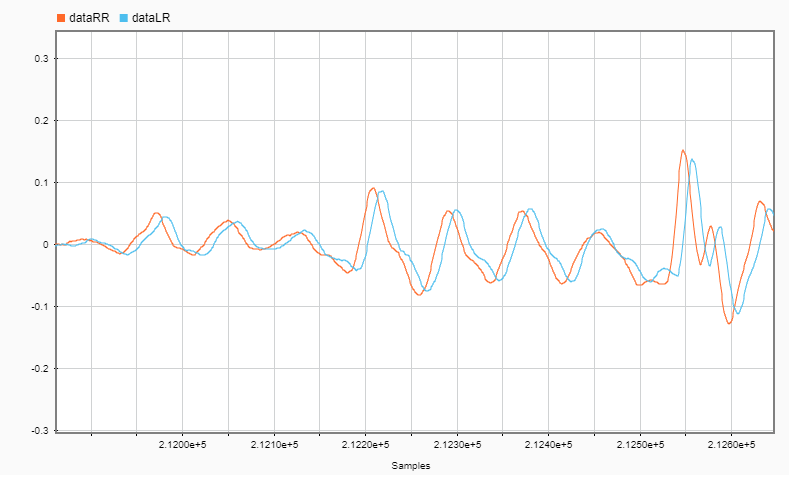
\includegraphics[width=0.8\textwidth]{Illustrations/DataR.png}
	\caption{Data from speaker in the right side}
	\label{fig:R}
\end{figure}

\begin{figure}[htp]
	\centering
	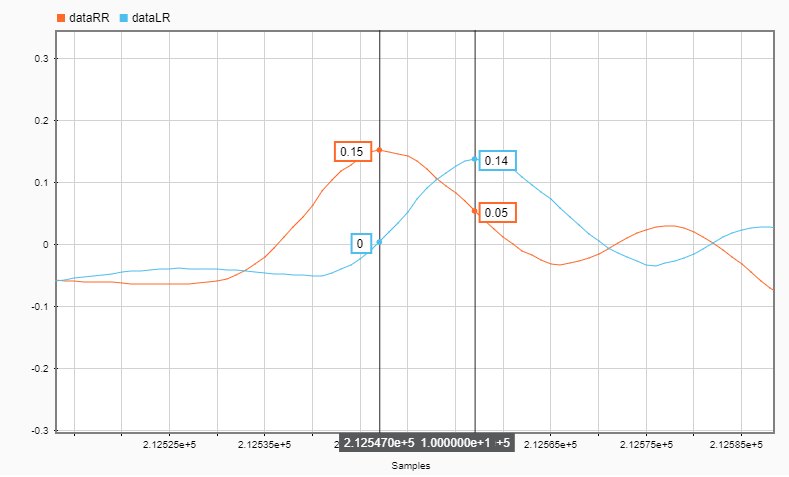
\includegraphics[width=0.8\textwidth]{Illustrations/DataR_with_Markers.png}
	\caption{Zoomed in data from speaker in the right side}
	\label{fig:closeR}
\end{figure}

 and when he spoke from the left, lift microphone was leading (Figures  \ref{fig:L}, \ref{fig:closeL})
 \todo[inline]{"For range -1 to 1 20*log10(x) corresponds to dB" Mention?}
 
 \begin{figure}[htp]
	\centering
	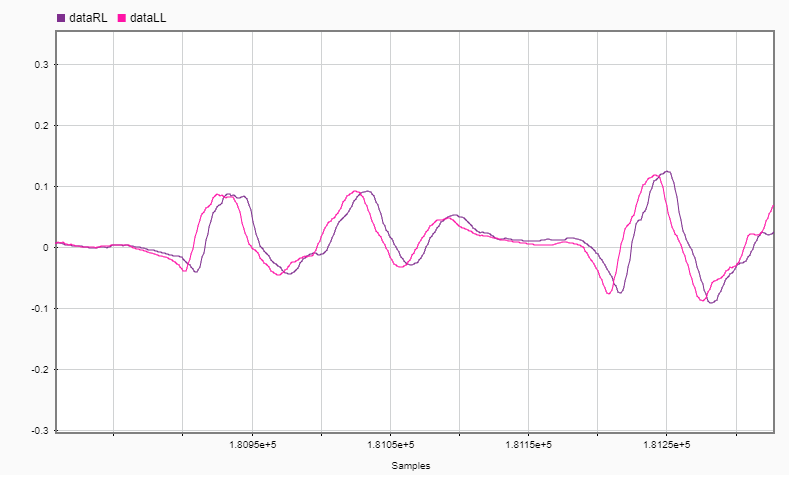
\includegraphics[width=0.8\textwidth]{Illustrations/DataL.png}
	\caption{Data from speaker in the left side}
	\label{fig:L}
\end{figure}

\begin{figure}[htp]
	\centering
	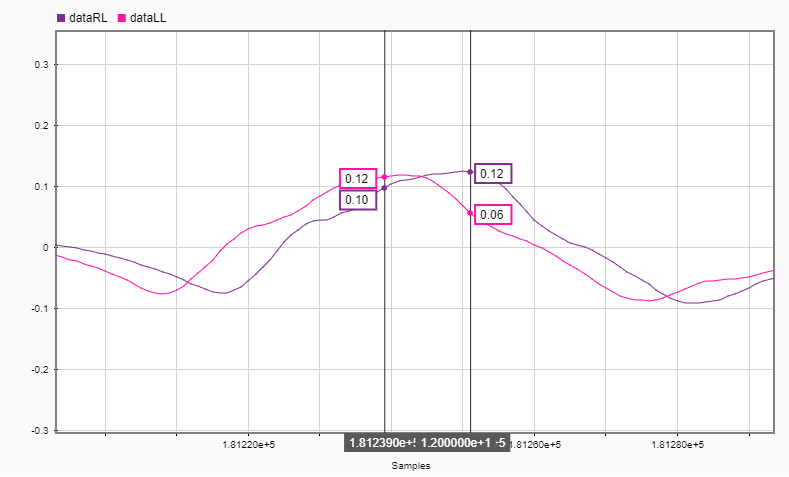
\includegraphics[width=0.8\textwidth]{Illustrations/DataL_with_Markers.png}
	\caption{Zoomed in data from speaker in the left side}
	\label{fig:closeL}
\end{figure}

\section{Conclusion}